\documentclass{article}
\usepackage{hyperref}
\usepackage{listings}
\usepackage{color}
\usepackage{xcolor}
\usepackage{geometry}
\usepackage{graphicx}
\usepackage{amsmath}
\usepackage{caption}
\usepackage{subcaption}
\usepackage{syntax}
\geometry{margin=1in}
\pdfminorversion=6

\newcommand\TODO[1]{\textcolor{red}{TODO: #1}}

\newcommand\header[2]{
    \begin{center}
        {\large
        UCSD CSE 291 (Differentiable Programming) Assignment #1: \\
        \vspace{0.3cm}
        \Large
        #2}
    \end{center}
}

\definecolor{dkgreen}{rgb}{0,0.6,0}
\definecolor{gray}{rgb}{0.5,0.5,0.5}
\definecolor{mauve}{rgb}{0.58,0,0.82}
\lstset{frame=tb,
        aboveskip=3mm,
        belowskip=3mm,
        showstringspaces=false,
        columns=flexible,
        basicstyle={\small\ttfamily},
        numbers=none,
        numberstyle=\tiny\color{gray},
        keywordstyle=\color{blue},
        commentstyle=\color{dkgreen},
        stringstyle=\color{mauve},
        breaklines=true,
        breakatwhitespace=true,
        tabsize=2
}

\hypersetup{colorlinks=true}


\begin{document}

\header{0}{Introduction to the \textbf{loma} Programming Language}

In this course, we will be using a C-like parallel programming language \textbf{loma} (invented for this course!). Our ultimate goal is to make loma ``differentiable'' and capable of automatically generating the derivatives of its code, and then use loma to implement your final project. In this handout, we will introduce the language and its compiler.

The design principles of loma are:
\begin{itemize}
    \item \textbf{Minimal}. To make implementing the compiler and the differentiation as simple as possible, we restrict as much language features as possible. As a result, the language lacks advanced object-oriented/functional features such as higher-order functions, subtyping or fancy type inference.
    \item \textbf{Differentiable}. Furthermore, to make differentiation possible/simpler/efficient, we impose restrictions to the language. For example, functions can only have one \lstinline{return} statement in the end, all \lstinline{while} loops need to have a static upper bound on the iteration size, recursion is not allowed, and there is no pointer. These restrictions will make more sense as you start to implement differentiation. As a result, loma is not Turing complete and can be seen as a domain-specific language -- this is a good thing as we can specialize the compiler to generate efficient code.
    \item \textbf{Static}. For efficiency purpose, to minimize dynamic memory allocation, loma's variables are all statically typed. In fact, all memory allocation inside loma needs to have size known at compile time. You can, however, allocate the memory dynamically outside of loma in the host code.
    \item \textbf{SIMD Parallel}. Loma programs will likely need to be executed in an optimization loop, either for machine learning, simulation, or inverse problems. These days it's not entirely practical to run these loops without any parallelism. Therefore, we need to be able to compile loma programs to vectorized CPU code or GPU code. Loma thus adopts a \href{https://en.wikipedia.org/wiki/Single_instruction,_multiple_data}{Single-Instruction-Multiple-Data} parallelism execution model.
    \item \textbf{Python embedding}. For ease of both scripting of loma programs and compiler development, loma is embedded in Python, and mostly follows Python's syntax. We aim for the syntax's familiarity and want to reuse Python's parser and AST modules (and existing syntax highlighters). Embedding in Python also makes it easy to use loma from a Python host code. Fortunately, loma should be much faster than Python in general since it's a compiled static type language and has GPU backends.
\end{itemize}

\section{Dependencies and requirements}

Loma requires Python version to be at least 3.10.14. 
Use \lstinline{pip install -r requirements.txt} to install the dependent packages.

\section{Hello, loma}

An example loma program looks like this (the file is located in \lstinline{examples/loma_code/sum_array.py}):
\begin{lstlisting}[language=python]
# sum_array.py
def sum_array(arr : In[Array[float]], arr_size : In[int]) -> float:
    i : int = 0
    s : float = 0.0
    while (i < arr_size, max_iter := 1000):
        s = s + arr[i]
        i = i + 1
    s_relu : float = 0.0
    if s > 0:
        s_relu = s
    return s_relu
\end{lstlisting}
Hopefully the code explains itself: it sums over an array, and returns the sum if the sum if larger than zero, otherwise it returns zero. A slightly peculiar syntax is that all while loops in loma needs to have an upper bound on the maximum iterations (\lstinline{max_iter}). We abused Python's named expression feature (recently added in Python 3.8!) for this annotation. The reason of the need for this annotation will be clearer when we get to the implementation of reverse-mode automatic differentiation for control flows in Homework 3. If we don't have the upper bound, then the differentiation requires us to have dynamic allocations, which is expensive on GPUs. Note that the maximum iteration is only an upper bound. The loop itself can still terminate before the maximum iteration count. Also note that despite the Python syntax, all variables have an explicit static type.

When you feed this program to the loma compiler and specifies C as a backend (currently, the two other available backends are ISPC and OpenCL, we will get to them later), the compiler will emit the following C code:
\begin{lstlisting}[language=c]
#include <math.h>
        
float sum_array(float* arr, int arr_size);
float sum_array(float* arr, int arr_size) {
    int i = (int)(0);
    float s = (float)(0.0);
    while ((i) < (arr_size)) {
        s = (s) + ((arr)[i]);
        i = (i) + ((int)(1));
    }
    float s_relu = (float)(0.0);
    if ((s) > ((int)(0))) {
        s_relu = s;
    } else {
    }
    return s_relu;
}
\end{lstlisting}

It then compiles the C code, loads it into a dynamic library (using \href{https://docs.python.org/3/library/ctypes.html}{ctypes}). You can compile and use this loma function in Python like this:
\begin{lstlisting}[language=python]
# sum_array_host.py
with open('loma_code/sum_array.py') as f:
    _, lib = compiler.compile(f.read(),
                              target = 'c',
                              output_filename = '_code/sum_array.so')

py_arr = [1.0, 2.0, 3.0, 4.0, 5.0]
arr = (ctypes.c_float * len(py_arr))(*py_arr)
assert abs(lib.sum_array(arr, len(py_arr)) - 15.0) < 1e-6
\end{lstlisting}
The host code is located in \lstinline{examples/sum_array_host.py}.

\section{Intermediate Representation}
\label{sec:IR}

The most important component of a programming language is its intermediate representation (IR). They are the data structures we use for representing a program and store important information. An IR is usually a directed graph. In our case, we further limit the graph to have no cycles (i.e., a directed acyclic graph, DAG). It's probably easiest to look at the IR to understand it. 
The IR of loma in the \href{https://en.wikipedia.org/wiki/Backus%E2%80%93Naur_form}{Backus-Naur Form} is:
\begin{grammar}
<func> ::= ('FunctionDef' <string> <arg>* <stmt>* <is_simd> <type>?
\alt 'ForwardDiff' <string> <string>
\alt 'ReverseDiff' <string> <string>) \\
'attributes' <int>?

<stmt> ::= ('Assign' <expr> <expr>
\alt 'Declare' <string> <type> [<expr>]? 
\alt 'Return' <expr>
\alt 'IfElse' <expr> <stmt>* <stmt>*
\alt 'While' <expr> <int> <stmt>*
\alt 'CallStmt' <expr>) \\
'attributes' <int>?

<expr> ::= ('Var' <string>
\alt 'ArrayAccess' <expr> <expr>
\alt 'StructAccess' <expr> <string>
\alt 'ConstFloat' <float>
\alt 'ConstInt' <int>
\alt 'BinaryOp' <bin_op> <expr> <expr>
\alt 'Call' <string> <expr>*) \\
'attributes' <int>? <type>?

<arg> ::= 'Arg' <string> <type> <inout>

<type> ::= 'Int'
\alt 'Float'
\alt 'Array' <type> <int>?
\alt 'Struct' <string> <struct_member>* <int>?
\alt 'Diff' <type>

<struct_member> ::= 'MemberDef' <string> <type>

<bin_op> ::= 'Add'
\alt 'Sub'
\alt 'Mul'
\alt 'Div'
\alt 'Less'
\alt 'LessEqual'
\alt 'Greater'
\alt 'GreaterEqual'
\alt 'Equal'
\alt 'And'
\alt 'Or'

<inout> ::= 'In' \alt 'Out'

<is_simd> :: 'True' \alt 'False'
\end{grammar}

If you have never seen anything like this, here is how to read it:
Each rule (\lstinline{::=}) defines how a symbol (e.g., \lstinline{<func>}) can be expanded. The first rule says a function definition \lstinline{<func>} consists of a \lstinline{<string>} (for the name of the function), zero or more arguments \lstinline{<arg>} (for the function arguments), zero or more statements \lstinline{<stmt>} (for the function body), a flag \lstinline{<is_simd>} (for whether the function is a SIMD kernel or not -- more about this later), and an optional return type. The \lstinline{|} character represents alternatives. For example, a statement \lstinline{<stmt>} can be either an assignment (\lstinline{'Assign'}), a variable declaration (\lstinline{'Declare'}), function return (\lstinline{'Return'}), if-else (\lstinline{'IfElse'}), or a while loop (\lstinline{'While'}). At the end of each statement we attached \lstinline{'attributes'} for extra information -- here we store the line number for error messages.

We will explain the more precise semantics of the IR later, but most of them should be self-explainable.

To implement the IR above, we represent it using ASDL (Abstract Syntax Definition Language) -- see \href{https://eli.thegreenplace.net/2014/06/04/using-asdl-to-describe-asts-in-compilers}{Eli Bendersky's blog post} for a brief introduction. This is what Python used for representing its \href{https://github.com/python/cpython/blob/main/Parser/Python.asdl}{abstract syntax tree}. The IR above can be directly translated to the following ASDL:
\begin{lstlisting}
    module loma {
      func = FunctionDef ( string id, arg* args, stmt* body, bool is_simd, type? ret_type )
           | ForwardDiff ( string id, string primal_func )
           | ReverseDiff ( string id, string primal_func )
             attributes  ( int? lineno )

      stmt = Assign     ( expr target, expr val )
           | Declare    ( string target, type t, expr? val )
           | Return     ( expr val )
           | IfElse     ( expr cond, stmt* then_stmts, stmt* else_stmts )
           | While      ( expr cond, int max_iter, stmt* body )
           | CallStmt   ( expr call )
           attributes   ( int? lineno )

      expr = Var          ( string id )
           | ArrayAccess  ( expr array, expr index )
           | StructAccess ( expr struct, string member_id )
           | ConstFloat   ( float val )
           | ConstInt     ( int val )
           | BinaryOp     ( bin_op op, expr left, expr right )
           | Call         ( string id, expr* args )
           attributes     ( int? lineno, type? t )

      arg  = Arg ( string id, type t, inout i )

      type = Int    ( )
           | Float  ( )
           | Array  ( type t, int? static_size )
           | Struct ( string id, struct_member* members, int? lineno )
           | Diff   ( type t )

      struct_member = MemberDef ( string id, type t )

      bin_op = Add()
             | Sub()
             | Mul()
             | Div()
             | Less()
             | LessEqual()
             | Greater()
             | GreaterEqual()
             | Equal()
             | And()
             | Or()

      inout = In() | Out()
    }
\end{lstlisting}
This IR is defined in \lstinline{ir.py} in the source code.

We then use a nice library written by \href{https://www.gilbertbernstein.com/}{Gilbert Bernstein} (see \lstinline{asdl_gen.py}) to convert the ASDL into a hierarchy of Python classes. For example, the \lstinline{stmt} ruleset above is converted to the following classes (code simplified a bit):
\begin{lstlisting}[language=python]
import attrs
from typing import Optional
# ...

class stmt:
  pass

@attrs.define(frozen=True)
class Assign(stmt):
    target: ref
    val: expr
    lineno: Optional[int] = None

@attrs.define(frozen=True)
class Declare(stmt):
    target: str
    t: type
    val: Optional[expr] = None
    lineno: Optional[int] = None

# ...
\end{lstlisting}
Hopefully you can see how the rest of the classes are constructed from the example above. When we run the loma compiler, the classes will be generated as a Python file in \lstinline{_asdl/loma.py}, where you can inspect these generated classes. 

Once we have these classes, we can then construct loma programs by composing objects of these classes. For example, the following code
\begin{lstlisting}[language=python]
x : int = y + 5
\end{lstlisting}
would be converted into the following loma IR:
\begin{lstlisting}[language=python]
Declare(target='x', t=Int(), val=Add(Var('y'), ConstInt(5)))
\end{lstlisting}

\section{Semantics.}
The meaning of the IR above follows a similar C program. We will explain the semantics through examples -- hopefully this is generalizable. You can also read \lstinline{codegen_c.py} as a reference.

\subsection{Function definition} 
The following \lstinline{FunctionDef} in loma IR
\begin{lstlisting}
FunctionDef(id='plus',
            args=(Arg(id='x', t=Int(), inout = In()),
                  Arg(id='y', t=Int(), inout = In()),
                  Arg(id='z', t=Array(t=Float(), static_size=None)), inout = In()),
                  Arg(id='w', t=Int(), inout = Out())
            body=(Return(val=ConstInt(val=0)),),
            is_simd=False,
            ret_type=Int())
\end{lstlisting}
(take some time to read it, it's not too bad), has the same meaning as the following C function definition:
\begin{lstlisting}[language=C]
int plus(int x, int y, float* z, int *w) {
    return 0;
}
\end{lstlisting}

Each function argument needs to be tagged either as an input (\lstinline{In()}) or an output (\lstinline{Out()}), and its type \lstinline{t} needs to be specified. If a function returns a value, the type of the returned value must also be specified. If a function does not return a value, then it's \lstinline{ret_type} is \lstinline{None}.

A function can take inputs and outputs that are of \lstinline{Array} types. You can have a struct of arrays or array of structs (or structs of arrays of structs). The function arguments are by default passed by values, except for arrays. When a callee modifies an array element, the caller will observe the changes.

If an argument is marked as \lstinline{In()}, you can never write to it. On the other hand, if an argument is marked as \lstinline{Out()}, you can never read from it. All arguments marked as \lstinline{Out()}, arrays or not, are passed by reference.

We will explain the \lstinline{is_simd} flag later when we talk about parallelization.

\lstinline{ForwardDiff} and \lstinline{ReverseDiff} are for the differentiation of the functions, and will be discussed in the later homework when we bump into them. 

\subsection{Types}

The type system of loma is similar to C except it's even simpler. The \lstinline{<type>} rule set above defines all the possible types in loma. There are only two primitive types: \lstinline{Int} and \lstinline{Float}. We can also define an \lstinline{Array} that is a list of the same type (the optional integer represents a fixed-size array). Finally, loma also supports \lstinline{Struct} (product types if you're a functional guru). We do not support sum types (e.g., unions in C) to make differentiation easy.

The \lstinline{Diff} type is for representing the differential of the type for automatic differentiation. We will explain it in the first homework.

\subsection{Statements}

\paragraph{Variable declaration.}
The following \lstinline{Declare} statement in loma IR
\begin{lstlisting}
Declare(target='x',
        t=Int(),
        val=ConstInt(val=5))
\end{lstlisting}
has the same meaning as the following C code
\begin{lstlisting}
int x = 5;
\end{lstlisting}

The \lstinline{val} part is optional. If it is \lstinline{None}, the variable is initialized to zero.

All the variable declaration needs to have a static size known at compile time. For example, a declaration of a struct object with an unbounded array member is not a valid loma program. \TODO{implement the check.}

\paragraph{Variable assignment.}
The following \lstinline{Assign} statement in loma IR
\begin{lstlisting}
Assign(target=RefName(id='x'),
       val=ConstInt(val=6))
\end{lstlisting}
has the same meaning as the following C code
\begin{lstlisting}
x = 6;
\end{lstlisting}
If \lstinline{x} is not declared before hand, this is an illegal loma program.

The target of the assign statement needs to be a \lstinline{ref}. A \lstinline{ref} can be a member of a struct or an element of an array. For example,
\begin{lstlisting}
Assign(target=RefArray(array=RefName(id='a'), index=ConstInt(val=1)),
       val=ConstInt(val=6))
Assign(target=RefStruct(struct=RefName(id='b'), member='c'),
       val=ConstInt(val=7))
\end{lstlisting}
means
\begin{lstlisting}
a[1] = 6;
b.c = 7;
\end{lstlisting}

The type of the target should match the right hand side, and the type cannot be an array or Struct (it can be access to the members of the array or the Struct). If the types of left hand side and right hand side are \lstinline{int} and \lstinline{float} respectively, our type checker automatically inserts a type casting operation \lstinline{float2int} or \lstinline{int2float} for the conversion.

\paragraph{Return.}
The following \lstinline{Return} statement in loma IR
\begin{lstlisting}
Return(val=ConstInt(val=0))
\end{lstlisting}
has the same meaning as the following C code
\begin{lstlisting}[language=c]
return 0;
\end{lstlisting}

To make differentiation easy, a \lstinline{Return} statement in loma IR can only be at the last statement, and can only appear once. \TODO{implement this}

\paragraph{Condition.}
The following \lstinline{IfElse} statement in loma IR
\begin{lstlisting}
IfElse(cond=BinaryOp(op=Greater(), left=Var(id='x'),
       right=ConstInt(val=0, lineno=4, t=None)),
       then_stmts=(Assign(target=RefName(id='y'), val=ConstInt(val=3)),),
       else_stmts=(Assign(target=RefName(id='z'), val=ConstInt(val=7)),))
\end{lstlisting}
has the same meaning as the following C code
\begin{lstlisting}[language=c]
if (x > 0) {
    y = 3;
} else {
    z = 7;
}
\end{lstlisting}

There is no \lstinline{else if} in loma IR. You can have an if statement inside the else statement. The else statement is optional.

\paragraph{While loops.}
The following \lstinline{While} statement in loma IR
\begin{lstlisting}
While(cond=BinaryOp(op=Less(), left=Var(id='i'),
      right=ConstInt(val=10)),
      max_iter=20,
      body=(Assign(target=RefName(id='i'), val=BinaryOp(op=Add(), left=Var(id='i'), right=ConstInt(val=1)),))
\end{lstlisting}
has the same meaning as the following C code
\begin{lstlisting}[language=c]
while (i < 10) {
    i = i + 1;
}
\end{lstlisting}
Notice that there is a \lstinline{max_iter} attribute in the loma while statement. It is an extra annotation of the while loop that specifies an upper bound of the number of iterations. This is a crucial information for the reverse-mode automatic differentiation we will implement in the homeworks. If we do not have the maximum iteration bounds, we will need dynamic memory allocations in reverse mode, leading to worse efficiency. Note that the upper bound can be loose -- like here, the loop always end in 10 steps, but we set the upper bound to be 20. If the upper bound is smaller than the actual loop iterations, the behavior of the program is undefined (it will likely crash when you perform reverse mode autodiff).

\paragraph{Call expressions.}
We will omit most of the specifications of expressions since it's very standard. Except for \lstinline{Call} which we provide a list of intrinsic functions. We have the follow list of intrinsic functions:

\begin{itemize}
\item \lstinline{sin(x : float) -> float}, \lstinline{cos(x : float) -> float}, \lstinline{exp(x: float) -> float}, \lstinline{log(x : float)}, \lstinline{pow(x : float, y : float) -> float}: standard math functions that takes \lstinline{float}(s) and returns a \lstinline{float}.
\item \lstinline{int2float(x : int) -> float}: type cast an integer to a float.
\item \lstinline{float2int(x : float) -> int}: type cast a float to an integer. The effect is the same as C typecasting, i.e., it will take the floor of the float.
\item \lstinline{thread_id() -> int}: for SIMD parallelism. Will be explained later.
\end{itemize}

\section{Frontend and Parsing}
As hinted at the beginning, loma is embedded in Python. That is, we borrow the Python syntax (but not the semantics), so that we can reuse Python's parser, and we can exploit on people's familiarity of Python's syntax. 

The frontend has an almost one-to-one relationship to the IR. Below we list how we translate the Python syntax to loma's IR: 

\subsection{Function definition.} 
The following Python frontend code:
\begin{lstlisting}[language=Python]
def plus(x : int, y : int, z : Array[float], w : Ref[int]) -> int:
\end{lstlisting}
will be translated to the following loma IR:
\begin{lstlisting}
FunctionDef(id='plus',
            args=(Arg(id='x', t=Int(), is_byref=False),
                  Arg(id='y', t=Int(), is_byref=False),
                  Arg(id='z', t=Array(t=Float(), static_size=None), is_byref=False),
                  Arg(id='w', t=Int(), is_byref=True)),
            body=None,
            is_simd=False,
            ret_type=Int())
\end{lstlisting}

\subsection{Statements.} 

\paragraph{Variable declaration.} This code
\begin{lstlisting}[language=Python]
x : int = 5
\end{lstlisting}
will be translated to:
\begin{lstlisting}
Declare(target='x',
        t=Int(),
        val=ConstInt(val=5))
\end{lstlisting}

The value part is optional. For example, you can write
\begin{lstlisting}[language=Python]
x : int
\end{lstlisting}
and it will be translated to
\begin{lstlisting}
Declare(target='x',
        t=Int(),
        val=None)
\end{lstlisting}

\paragraph{Variable assignment.} This code
\begin{lstlisting}[language=Python]
x = 6
\end{lstlisting}
will be translated to
\begin{lstlisting}
Assign(target=RefName(id='x'),
       val=ConstInt(val=6))
\end{lstlisting}

Note that in loma, \lstinline{x : int = 5} and \lstinline{x = 5} are two different statements, while in Python they are the same.

\paragraph{Return.} This code
\begin{lstlisting}[language=Python]
return 0
\end{lstlisting}
will be translated to
\begin{lstlisting}
Return(val=ConstInt(val=0))
\end{lstlisting}

\paragraph{If statements.} This code
\begin{lstlisting}[language=c]
if (x > 0):
    y = 3
else:
    z = 7
\end{lstlisting}
will be translated to
\begin{lstlisting}
IfElse(cond=BinaryOp(op=Greater(), left=Var(id='x'),
       right=ConstInt(val=0, lineno=4, t=None)),
       then_stmts=(Assign(target=RefName(id='y'), val=ConstInt(val=3)),),
       else_stmts=(Assign(target=RefName(id='z'), val=ConstInt(val=7)),))
\end{lstlisting}

Our frontend does not support \lstinline{elif} in Python.

\paragraph{While loops.} This code
\begin{lstlisting}[language=python]
while (i < 10, max_iter := 20):
    i = i + 1
\end{lstlisting}
will be translated to
\begin{lstlisting}
While(cond=BinaryOp(op=Less(), left=Var(id='i'),
      right=ConstInt(val=10)),
      max_iter=20,
      body=(Assign(target=RefName(id='i'), val=BinaryOp(op=Add(), left=Var(id='i'), right=ConstInt(val=1)),))
\end{lstlisting}

\subsection{Struct definitions}
Following class definitions in Python
\begin{lstlisting}[language=Python]
class Foo:
    x : int
    bar : Bar

class Bar:
    y : float
    z : int
\end{lstlisting}
will be translated to
\begin{lstlisting}
Struct(id='Foo', members=(MemberDef(id='x', t=Int()), MemberDef(id='bar', t=Struct(id='Bar', members=()))))
Struct(id='Bar', members=(MemberDef(id='y', t=Float()), MemberDef(id='z', t=Int())))
\end{lstlisting}

\subsection{Implementation}

To implement the translation above, we use the \lstinline{ast} package in Python and build a \href{https://en.wikipedia.org/wiki/Recursive_descent_parser}{recursive descent parser}. See \lstinline{parser.py} for more details.

For example, in the Python frontend, the top level definition can either be a \lstinline{ast.ClassDef} or a \lstinline{ast.FunctionDef}. So we parse them using the following code:
\begin{lstlisting}[language=Python]
def parse(code : str) -> tuple[dict[str, loma_ir.Struct], dict[str, loma_ir.func]]:
    """ Given a loma frontend code represented as a string,
        convert the code to loma IR.
        Returns both the parsed loma Structs and functions.
    """

    module = ast.parse(code)
    structs = {}
    for d in module.body:
        if isinstance(d, ast.ClassDef):
            s = visit_ClassDef(d)
            structs[s.id] = s

    funcs = {}
    for d in module.body:
        if isinstance(d, ast.FunctionDef):
            f = visit_FunctionDef(d)
            funcs[f.id] = f
        elif isinstance(d, ast.Assign):
            f = visit_Differentiate(d)
            funcs[f.id] = f

    return structs, funcs
\end{lstlisting}

The \lstinline{parse} function then relies on \lstinline{visit_ClassDef} and \lstinline{visit_FunctionDef}:
\begin{lstlisting}[language=Python]
def visit_ClassDef(node) -> loma_ir.Struct:
    """ Given a Python AST node representing a class definition,
        convert to a loma Struct.

        e.g.,
        class Foo:
            x : int
            y : float
    """

    members = []
    for member in node.body:
        match member:
            case ast.AnnAssign():
                assert isinstance(member.target, ast.Name)
                t = annotation_to_type(member.annotation)
                members.append(loma_ir.MemberDef(member.target.id, t))
            case _:
                assert False, f'Unknown class member statement {type(member).__name__}'
    return loma_ir.Struct(node.name, members, lineno = node.lineno)

def visit_FunctionDef(node) -> loma_ir.FunctionDef:
    """ Given a Python AST node representing
        a function definition,
        convert to the corresponding loma
        FunctionDef.
    """

    node_args = node.args
    assert node_args.vararg is None
    assert node_args.kwarg is None
    args = [loma_ir.Arg(arg.arg,
                        annotation_to_type(arg.annotation),
                        annotation_to_inout(arg.annotation)) for arg in node_args.args]
    body = [visit_stmt(b) for b in node.body]
    ret_type = None
    if node.returns:
        ret_type = annotation_to_type(node.returns)

    is_simd = False
    for decorator in node.decorator_list:
        if isinstance(decorator, ast.Name):
            if decorator.id == 'simd':
                is_simd = True

    return loma_ir.FunctionDef(node.name,
                               args,
                               body,
                               is_simd,
                               ret_type = ret_type,
                               lineno = node.lineno)
\end{lstlisting}

\section{Type and semantic checks}
After the parsing, the compiler will go through a type and semantic analysis phase. The code is mostly in \lstinline{check.py} and \lstinline{type_inference.py}. The entry point is the \lstinline{check_ir} function in \lstinline{check.py}:

\TODO{update this code snippet after we implement more checking.}
\begin{lstlisting}[language=Python]
def check_ir(structs : dict[str, loma_ir.Struct],
             diff_structs : dict[str, loma_ir.Struct],
             funcs : dict[str, loma_ir.func],
             check_diff : bool):
    """ Performs checks and type inferences on the loma functions (funcs).
        Fill in the type information of expressions.
        Raise errors when we see illegal code.

        Parameters:
        structs - a dictionary that maps the ID of a Struct to 
                the corresponding Struct
        diff_structs - a dictionary that maps the ID of the primal
                Struct to the corresponding differential Struct
                e.g., diff_structs['float'] returns _dfloat
        funcs - a dictionary that maps the ID of a function to 
                the corresponding func
        check_diff - whether we perform check_unhandled_differentiation
                     or not.
    """

    for f in funcs.values():
        if check_diff:
            check_unhandled_differentiation(f)
        check_duplicate_declare(f)
        check_undeclared_vars(f)

    type_inference.check_and_infer_types(structs, diff_structs, funcs)
\end{lstlisting}

The most important part is the type inference and checking phase: \lstinline{type_inference.check_and_infer_types}. The rest mostly just checking obvious erros like duplicate variables declaration.

The type inferencer and checker go through all functions, fill in the type information, and check if the types match in each statement:
\begin{lstlisting}[language=Python]
def check_and_infer_types(structs : dict[str, loma_ir.Struct],
                          diff_structs : dict[str, loma_ir.Struct],
                          funcs : dict[str, loma_ir.func]):
    for id, f in funcs.items():
        ti = TypeInferencer(structs, diff_structs, funcs)
        funcs[id] = ti.mutate_function(f)
\end{lstlisting}

The \lstinline{TypeInferencer} class inherits from an \lstinline{IRMutator} class that we use to trasnform code:
\begin{lstlisting}[language=Python]
class TypeInferencer(irmutator.IRMutator):
    # ...
\end{lstlisting}

The \lstinline{IRMutator} class is the base class that we will also use repeatedly through the class. It essentially implements the ``Visitor pattern'' where we can visit an IR node and all its children recursively. For example, the \lstinline{mutate_function_def} function in \lstinline{IRMutator} looks like this:
\begin{lstlisting}[language=Python]
def mutate_function_def(self, node):
    new_body = [self.mutate_stmt(stmt) for stmt in node.body]
    # Important: mutate_stmt can return a list of statements. We need to flatten the list.
    new_body = flatten(new_body)
    return loma_ir.FunctionDef(\
        node.id, node.args, new_body, node.is_simd, node.ret_type, lineno = node.lineno)
\end{lstlisting}
It recursively calls the \lstinline{mutate_stmt} function and assemble a new \lstinline{FunctionDef} that accounts for the new mutations. Note that, as commented, \lstinline{mutate_stmt} can sometimes return a list of statement, thus we need to unpack the list.

The \lstinline{TypeInferencer} then overrides the all the mutations to infer the types, check them, and throw errors when types do not match.

After the type inference phase, the \lstinline{.t} attribute for each expression (\lstinline{expr}) is filled.

\section{C Backend}

Given a loma program, we will ``lower'' it to a target language in the backends. Currently loma supports three backends: C, \href{https://ispc.github.io/index.html}{ispc}, and OpenCL. Let's talk about the C backend here, and we will discuss ispc and OpenCL backends after we discuss the parallelization model of loma.

Similar to \lstinline{IRMutator}, we also have an \lstinline{IRVisitor} that simply recursively visits the IR nodes without mutating them.

To transform a program, we recursively visit the IR nodes using an \lstinline{IRVisitor}:
\begin{lstlisting}[language=python]
class CCodegenVisitor(visitor.IRVisitor):
    code = ''
    tab_count = 0

    # ...
\end{lstlisting}

For example, following is the visit member function for a while loop:
\begin{lstlisting}[language=python]
def visit_while(self, loop):
    self.emit_tabs()
    self.code += f'while ({self.visit_expr(loop.cond)}) {{\n'
    self.tab_count += 1
    for stmt in loop.body:
        self.visit_stmt(stmt)
    self.tab_count -= 1
    self.emit_tabs()
    self.code += '}\n'
\end{lstlisting}

We recursively visit the conditions and body statements using other visit functions, and append the generated code to \lstinline{self.code}.

The translation straightforwardly follows the program semantics discussed in Section~\ref{sec:IR}.

The compiled C functions are compatible with \href{https://docs.python.org/3/library/ctypes.html}{ctypes}. You can call the functions in the Python host code like the following:
\begin{lstlisting}[language=python]
# foo.py
class Foo:
    arr : Array[int]

def foo(f : In[Foo], g : int) -> int:
    return f.arr[0] + f.arr[1] + g

# host code
with open('foo.py') as f:
    structs, lib = compiler.compile(f.read(),
                                    target = 'c',
                                    output_filename = '_code/foo.so')
py_arr = [1, 2]
arr = (ctypes.c_int * len(py_arr))(*py_arr)
Foo = structs['Foo']
f = Foo(arr=arr)
assert lib.foo(f, 3) == 6
\end{lstlisting}

The \lstinline{compile} function returns both a dictionary of \lstinline{structs}, and a ctypes library \lstinline{lib}. The \lstinline{structs} dictionary contains all of the ctypes structs indexed by name. You can then use them to assemble the function arguments and call the function to get the results.

\section{SIMD Parallelism and the OpenCL backend}

As mentioned, to use loma in practice, it's more or less necessary these days to support some form of parallelism. We adopt a SIMD parallelism model similar to how CUDA and OpenCL work. For example, the following loma program parallely adds two integer arrays \lstinline{x} and \lstinline{y} and store the results into the array \lstinline{z}.
\begin{lstlisting}[language=python] 
@simd
def parallel_add(x : In[Array[int]],
                 y : In[Array[int]],
                 z : Out[Array[int]]):
    i : int = thread_id()
    z[i] = x[i] + y[i]
\end{lstlisting}

Effectively, the semantics of this function is equivalent to the following program with a parallel for loop at the outmost:
\begin{lstlisting}[language=c]
void parallel_add(int *x, int *y, int *z, int n) {
    /* runs in parallel */
    for (int thread_id = 0; thread_id < n; i++) {
        int i = thread_id;
        z[i] = x[i] + y[i];
    }
}
\end{lstlisting}
Note that the number of threads \lstinline{n} is lifted to an extra argument of the function.

If compiling using the C backend, loma generates the equivalent C code to above and simulate the parallelism serially. More interesting things happen if we specify other backends. Specifically, loma supports two other backends: \href{https://ispc.github.io/}{ISPC} and OpenCL. We'll focus the discussion on the OpenCL backend, but the ISPC backend works similarly (read the ISPC documentation in their webpage if you're interested in it).

The loma code above would be translated into the following OpenCL code.
\begin{lstlisting}[language=c]
__kernel void parallel_add(__global int* x, __global int* y, __global int* z) {
    int i = get_global_id(0);
    z[i] = x[i] + y[i];
}
\end{lstlisting}

The only differences are the two extra keywords: \lstinline{__kernel}, \lstinline{__global} and the function for getting thread id: \lstinline{get_global_id()}. 

In OpenCL, \lstinline{__kernel} marks a function as a SIMD function (similar to the \lstinline{@simd} decorator in loma). This allows a host program outside of OpenCL to call the kernel. Functions not marked as kernel can only be called by functions inside the same OpenCL program. The \lstinline{__global} keyword marks an argument to be pointing to a global memory pool (e.g., the GPU global memory). The \lstinline{get_global_id} function, expectedly, get the ID of the current thread, and the argument \lstinline{0} specifies the dimension of the workers, which in our case is irrelevant since we always launch threads in a single dimension. 

As you can see, the generation of a OpenCL kernel is basically the same as a C code, so we can inherit most of our C generation code. See \lstinline{codegen_opencl.py} for reference.

Calling the OpenCL kernel from our Python host code is more complicated though. Following is the code:
\begin{lstlisting}[language=python]
cl_ctx, cl_device, cl_cmd_queue = cl_utils.create_context()

with open('loma_code/parallel_add.py') as f:
    structs, lib = compiler.compile(f.read(),
                                    target = 'opencl',
                                    opencl_context = cl_ctx,
                                    opencl_device = cl_device,
                                    opencl_command_queue = cl_cmd_queue)
py_x = [2, 3, 5]
x = (ctypes.c_int * len(py_x))(*py_x)
py_y = [7, 11, 13]
y = (ctypes.c_int * len(py_y))(*py_y)
py_z = [0, 0, 0]
z = (ctypes.c_int * len(py_z))(*py_z)

status = ctypes.c_int32()
bufx = cl.clCreateBuffer(cl_ctx,
                         cl.CL_MEM_READ_ONLY | cl.CL_MEM_COPY_HOST_PTR,
                         ctypes.sizeof(x),
                         ctypes.byref(x),
                         ctypes.byref(status))
cl_utils.cl_check(status.value)
bufy = cl.clCreateBuffer(cl_ctx,
                         cl.CL_MEM_READ_ONLY | cl.CL_MEM_COPY_HOST_PTR,
                         ctypes.sizeof(y),
                         ctypes.byref(y),
                         ctypes.byref(status))
cl_utils.cl_check(status.value)
bufz = cl.clCreateBuffer(cl_ctx,
                         cl.CL_MEM_WRITE_ONLY,
                         ctypes.sizeof(z),
                         None,
                         ctypes.byref(status))
cl_utils.cl_check(status.value)

lib.parallel_add(bufx, bufy, bufz, len(py_z))
cl.clFinish(cl_cmd_queue)

cl.clEnqueueReadBuffer(cl_cmd_queue,
                       bufz,
                       cl.CL_TRUE,
                       0,
                       ctypes.sizeof(z),
                       ctypes.byref(z),
                       0,
                       None,
                       None)

assert z[0] == 9 and z[1] == 14 and z[2] == 18
\end{lstlisting}
We use the wonderful library \href{https://github.com/tinygrad/gpuctypes}{gpuctypes} from geohot for wrapping OpenCL APIs in Python. We then abstract some of the OpenCL functions in \lstinline{cl_utils.py}. Let's look at the code line by line:
\begin{lstlisting}[language=python]
cl_ctx, cl_device, cl_cmd_queue = cl_utils.create_context()
\end{lstlisting}
This line creates a OpenCL ``context'', selects the relevant device (CPU or GPU or something else), and creates a command queue we can use to launch the kernels. To select a device, by default the function asks the user interactively like the following:
\begin{lstlisting}
Choose platform:
[0] b'Apple'
Choice [0]:0

Choose device:
[0] b'Intel(R) Core(TM) i7-9750H CPU @ 2.60GHz'
[1] b'Intel(R) UHD Graphics 630'
[2] b'AMD Radeon Pro 5300M Compute Engine'
Choice [0]:2

Set the environment variable OPENCL_CTX='0:2' to avoid being asked again.
\end{lstlisting}
Here, we choose our device to be the AMD GPU on my Apple machine.

The lines 
\begin{lstlisting}[language=python]
with open('loma_code/parallel_add.py') as f:
    structs, lib = compiler.compile(f.read(),
                                    target = 'opencl',
                                    opencl_context = cl_ctx,
                                    opencl_device = cl_device,
                                    opencl_command_queue = cl_cmd_queue)
py_x = [2, 3, 5]
x = (ctypes.c_int * len(py_x))(*py_x)
py_y = [7, 11, 13]
y = (ctypes.c_int * len(py_y))(*py_y)
py_z = [0, 0, 0]
z = (ctypes.c_int * len(py_z))(*py_z)
\end{lstlisting}
are similar to the C backend.

Next, we create the OpenCL buffers for the inputs and outputs:
\begin{lstlisting}[language=python]
status = ctypes.c_int32()
bufx = cl.clCreateBuffer(cl_ctx,
                         cl.CL_MEM_READ_ONLY | cl.CL_MEM_COPY_HOST_PTR,
                         ctypes.sizeof(x),
                         ctypes.byref(x),
                         ctypes.byref(status))
cl_utils.cl_check(status.value)
bufy = cl.clCreateBuffer(cl_ctx,
                         cl.CL_MEM_READ_ONLY | cl.CL_MEM_COPY_HOST_PTR,
                         ctypes.sizeof(y),
                         ctypes.byref(y),
                         ctypes.byref(status))
cl_utils.cl_check(status.value)
bufz = cl.clCreateBuffer(cl_ctx,
                         cl.CL_MEM_WRITE_ONLY,
                         ctypes.sizeof(z),
                         None,
                         ctypes.byref(status))
cl_utils.cl_check(status.value)
\end{lstlisting}
We use \lstinline{cl_utils.cl_check} to check whether the buffer creation has succeed or not.

Next, we launch the kernel (the kernel launching is encapsulated in a class \lstinline{OpenCLKernel} in \lstinline{cl_utils.py}.), and wait for the kernel to finish computation.
\begin{lstlisting}[language=python]
lib.parallel_add(bufx, bufy, bufz, len(py_z))
cl.clFinish(cl_cmd_queue)
\end{lstlisting}

Lastly, we read from the buffer (potentially copy the results from GPU to CPU) and compare the expected results.
\begin{lstlisting}[language=python]
cl.clEnqueueReadBuffer(cl_cmd_queue,
                       bufz,
                       cl.CL_TRUE,
                       0,
                       ctypes.sizeof(z),
                       ctypes.byref(z),
                       0,
                       None,
                       None)

assert z[0] == 9 and z[1] == 14 and z[2] == 18
\end{lstlisting}

\section{An example of a small ray tracer}
\begin{figure}
\centering
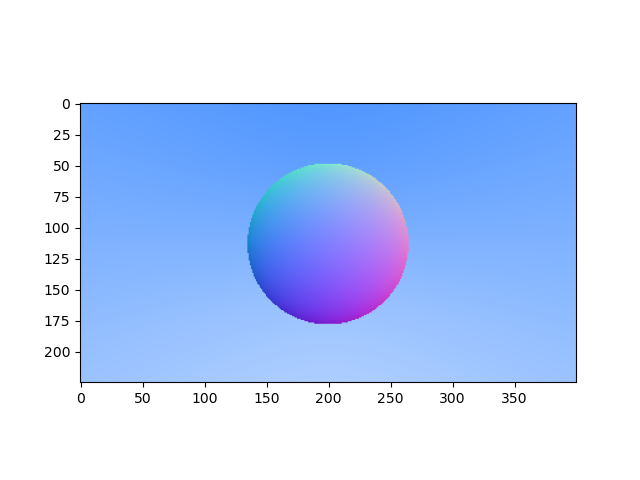
\includegraphics[width=0.8\linewidth]{imgs/raytrace.png}
\vspace{-20pt}
\caption{An image generated by a ray tracer implemented using loma.}
\label{fig:raytrace}
\end{figure}

\lstinline{examples/raytrace_host.py} and \lstinline{examples/loma_code/raytrace.py} shows the loma implementation of a simple ray tracer (code mostly taken from \href{https://raytracing.github.io/books/RayTracingInOneWeekend.html}{Ray Tracing in One Weekend}). Figure~\ref{fig:raytrace} shows the image rendered by the ray tracer. It also shows how loma interacts with numpy code.

\end{document}
